\chapter{\uppercase{Location Prediction}}

Based on the questions we answered in the previous section, we have enough
information to build a system for location prediction, which we call
FriendlyLocation.
Since the location prediction system will be run on a large number of of users,
it must be fast and scalable.

\section{Edge Length Prediction}

Before we predict a user's location, we need a way to estimate the probability
that a geo-located user is at a location given the position of their contact.
%
To achieve this, we trained a regression tree to predict the distance between a
user and a contact.
%
The regression tree was trained on several of the features from the previous
section that are correlated with users living near each other:
\begin{itemize}
\item the type of contact
\item if the geo-located user mentioned the contact
\item if the contact had a protected account
\item the contact's follower count
\item the quality of the contact's lactation
\item the contact's local contact ratio
\end{itemize}
%
Since the distances between users varied by several orders of magnitude, we
trained the regressor to predict the log of the distance.
%
The tree regressor was configured to not split leafs with fewer than 1000 data
points to prevent over-fitting.
% FIXME: this needs more, but I'm not sure what.


\section{Model}
\label{sec:model}

In this section, we build a model for the probability that a user, who we refer
to as the target user, lives at a specific location given the approximate
location of his contacts.
%
In the previous sections, we looked at the probability that a contact lived a
certain distance from a given user.
%
Location prediction requires the probability that the user lives at a specific
location.


\begin{figure}[tb]
\centering
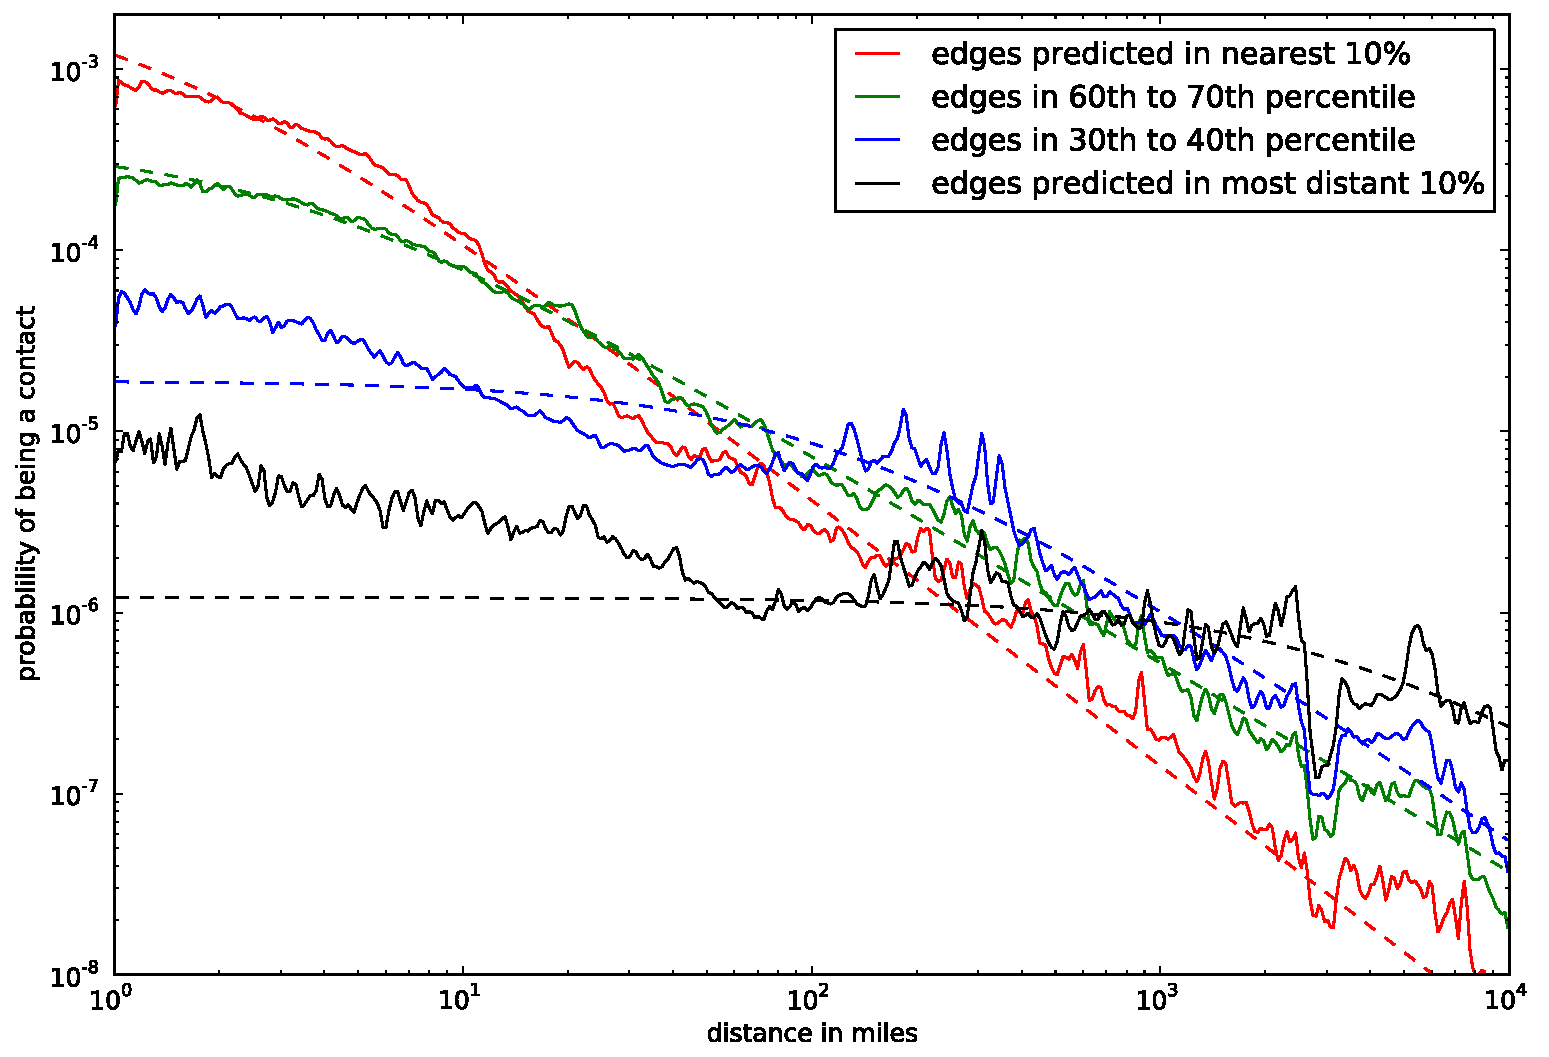
\includegraphics[width=\linewidth]{figures/near_prob_fit.pdf}
\caption{
After splitting edges into groups based their predicted distance, each group was fit to a curve. Here are four of the ten curves.
}
\label{fig:NearProbFit}
\end{figure}

First, we needed a model for the density of Twitter users.
\[
    pContact(group,dist) = \frac{nebrEdges(group,dist)}{strangeEdges(dist) \times numberGroups}
\]

We calculated the distance between every geo-located user and every contact
(even for contacts and users who had no relationship).
%
In order to speed up this calculation, we divided the world into a \.1 degree
by \.1 degree grid, and counted the number of of contacts in each of the spots
on the grid.
%
We took the distances between users and sorted them into 360 logarithmically
scaled bins between 10 miles and 10,000 miles.
%
(Every edge less than 10 miles was ignored because it was around the size of
the grid boxes, and therefore, noisy. Distances greater than 10,000 miles are
on the opposite side of the world.)
%
We fit this segment to a power law curve, which gives us a way to estimate
strangeEdges.

% Put more about fit_stgrs
The edges were sorted by the distance that the tree regressor predicted and
split into ten equal groups.
%
We split the edges in these groups into 480 logarithmically-scaled bins from 1
to 10,000 miles based on the length of the edge.
%
We divided the number of edges that actually existed at each distance by the
number of edges that could have existed as predicted by strangeEdges.
%
We fit it to this curve:
%
\[
pContact(group, dist) = a_{group} \times (b_{group}+dist)^{-c_{group}}
\]

Four of the ten curves from one of the five evaluation groups and their lines
of best fit are shown in Figure~\ref{fig:NearProbFit}.
%
The best contacts are orders of magnitude more
likely to live near a target user than the worst contacts.
%
If the predictions from the tree regressor were ignored, and users were placed
into one group instead of ten equal groups, this would reduce to the model
for friendship and distance presented in \cite{backstrom2010find}.


\section{System}
We used this model to build a Maximum Likelihood Estimator.


We use this to create a simple procedure for estimating the location for a user:
\begin{enumerate}
\item Randomly pick up to 25 of the user's contacts.
\item For each of those contacts:
\begin{enumerate}
    \item Geocode the location field and calculate the the predicted error.
    \item Ignore the contact if they have no decodable location information.
    Approximately one third of the contacts are ignored.
    \item Use the regression tree to estimate the length of the edge.
    \item Determine which of the ten groups this edge is in to find the curve
        for the probability that the contact lives near the
\end{enumerate}
\item For each of the contacts' locations calculate the probability that the
target user lives at that location using the maximum likelihood estimator.
\item FIXME: (For some versions we added in UTC offset, reported location, and stranger prob)
\item Pick the location with the highest probability.
\end{enumerate}

FIXME: formula for MLE, and description
FIXME: more here

